
    \begin{abstract_online}{Electronic Properties and High $\mathbf{CO_2}$ Capture Ability of Two-Dimensional Metal Nitrides($\mathbf{XN}$; $\mathbf{X = Al, Ga, In}$): A Computational Study}{%
        \underline{S. H. Mir}$^{1}$, J. K. Singh$^{2}$}{%
        }{%
        $^1$ Department of Chemistry, IIT Kanpur, India\newline{}$^2$ Department of Chemical Engineering, IIT Kanpur, India}
    Developing highly efficient sorbent materials for $CO_2$ separation and capture from flue gas mixture is most important for reducing impact of $CO_2$ on the environment [1]. On the basis of density functional theory calculations with dispersion correction [2,3], we performed ab initio calculations to investigate the structural stability, carrier mobility, and $CO_2$ separation and capture ability of mono-layered group III nitrides (XN) for $CO_2$ capture. The results showed that the studied two-dimensional sheets exhibit indirect band gaps, ranging from 0.59 eV for InN to 2.91 eV for AlN predicted using PBE functional [4] as shown in Figure 1. Mobility calculations performed using deformation potential theory shows that the mobility is dominated by holes as compared to electrons and reaches a value of $1.7 \times 10^3 cm^2 V^{−1} s^{−1}$ for AlN. The order of the hole mobility follows as $AlN \ > \ GaN \ > \ InN$. Density functional perturbation theory was used to predict the frequency of Raman active modes, the results showed a red shift in the calculated Raman peak frequency with increase in the mass of metal ion. The calculated adsorption energy of $CO_2$ is in the range of -0.17 eV to $-0.41 \ eV$ for XN. The adsorption energy of $CO_2$ on various nanostructures follows the order as $EGaN \ > \  EInN \ > \ EalN$. On the other hand, it is seen that $N_2$ shows significantly weaker interaction with the surfaces of XN as compared to $CO_2$, indicating high selectivity of sheets towards $CO_2$ capture. \begin{center}  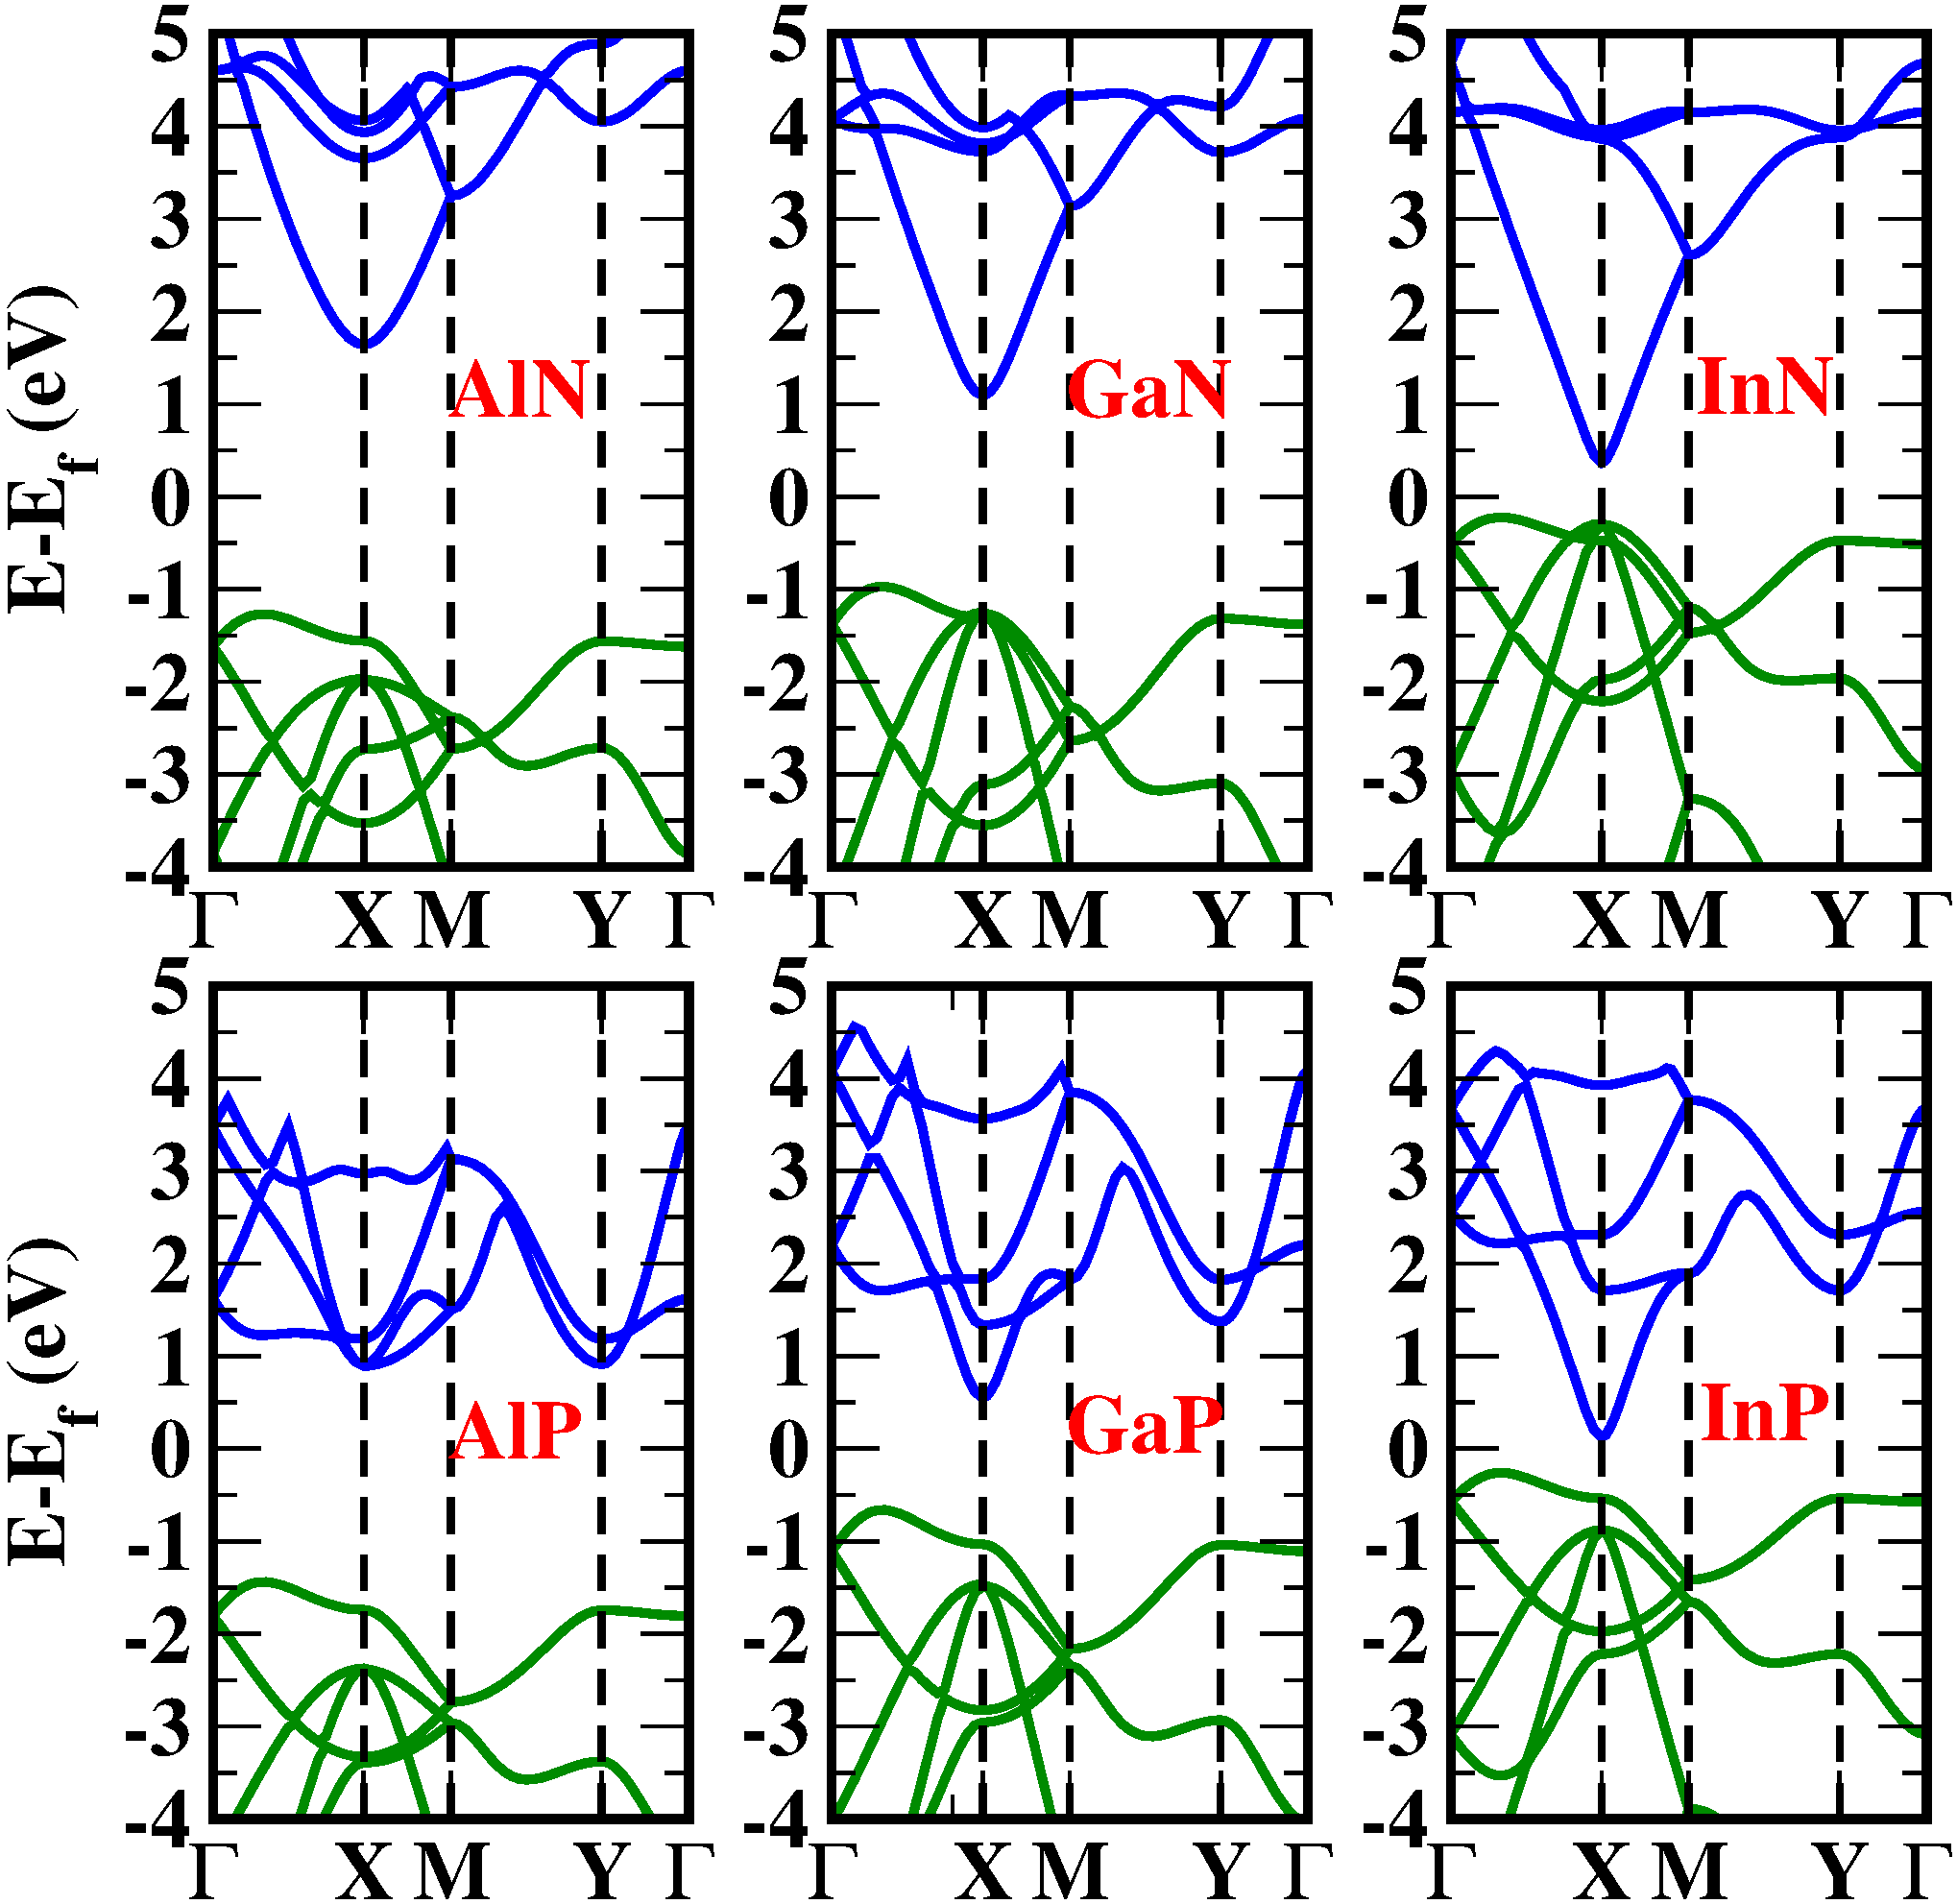
\includegraphics[width=0.95\linewidth]{abstracts/txt/figures/showkat.png}  \caption{\textbf{Figure 1:} Band structure of metal nitrides.}  \end{center} 
    
        \textbf{References} \newline{}[1] J. Phys. Chem. C 2015, 119, 6912−6917.\newline{}[2] J. Phys.: Condens. Matter 2009, 21, 395502.\newline{}[3] Phys. rev. Lett. 1996, 77, 3865.\newline{}[4] J. Chem. Phys. 2010, 132, 154104.
    \end{abstract_online}
    